\uuid{AKnT}
\chapitre{Autre}
\niveau{L3}
\module{Topologie}
\sousChapitre{Autre}
\titre{ Classification linéaire par un perceptron }
\theme{réseaux de neurones}
\auteur{ Maxime NGUYEN }
\datecreate{2024-11-17}
\organisation{ AMSCC }

\difficulte{}
\contenu{
	\question{ Décrire un perceptron qui permet de réaliser la classification entre les points bleus et les points rouges comme dans le graphique ci-dessous. 
\begin{center}
	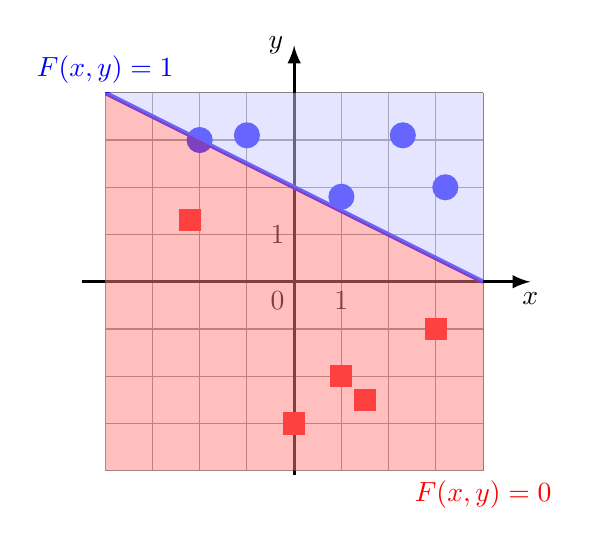
\begin{tikzpicture}[scale=0.6]
		\tikzstyle{rouge} = [fill,rectangle,red,scale=1.2];
		\tikzstyle{bleu} = [fill,circle,blue] ;
		
		\draw[gray] (-4,-4) grid ++(8,8);
		\draw[->,>=latex, very thick,black] (-4.5,0)--(5,0) node[below] {$x$};
		\draw[->,>=latex, very thick, black] (0,-4.1)--(0,5) node[left] {$y$};
		
		\node[below left] at (0,0) {$0$};
		\node[left] at (0,1) {$1$};
		\node[below] at (1,0) {$1$};
		
		\foreach \x/\y in {-2/3,3.2/2,-1/3.1,1/1.8,2.3/3.1}{
			\node[bleu] at (\x,\y) {};
		}
		\foreach \x/\y in {1/-2,3/-1,1.5/-2.5,0/-3,-2.2/1.3}{
			\node[rouge] at (\x,\y) {};
		}
		
		\begin{scope}[even odd rule]
			\clip (-4,-4) rectangle (4,4);
			\draw[blue,ultra thick] (-4,4) -- (4,0);
			\fill[red!50,opacity=0.5] (-4,4) -- (-4,-4) --(4,-4)--(4,0) -- cycle;
			\fill[blue!20,opacity=0.5] (-4,4) -- (-4,4) --(4,4)--(4,0) -- cycle;
			
		\end{scope}
		
		\node[scale=1,red,below] at (4,-4) {$F(x,y)=0$};
		\node[scale=1,blue,above] at (-4,4) {$F(x,y)=1$};
		%\node[red,below] at (-1,-4) {$y=8x+4$};
		
	\end{tikzpicture}
\end{center} }
}